% *******************************************************************************
% * Copyright (c) 2007 by Elexis
% * All rights reserved. This document and the accompanying materials
% * are made available under the terms of the Eclipse Public License v1.0
% * which accompanies this distribution, and is available at
% * http://www.eclipse.org/legal/epl-v10.html
% *
% *  $Id: agenda.tex 4902 2009-01-03 10:47:34Z rgw_ch $
% *******************************************************************************
% !Mode:: "TeX:UTF-8" (encoding info for WinEdt)

\section{Elexis-Agenda}\label{Agenda}
\index{Termin} Mehrbenutzerfähige Agenda zum Einbinden in Elexis. Dieses Plugin
ist Teil der Standard-Distribution.
Dieser Artikel beschreibt die Konfiguration und Verwendung der Agenda.
\subsection{Konfiguration}


Wählen Sie im Menü \textbf{Datei -Einstellungen}. Wenn das Agenda-Plugin installiert ist,
findet sich dort eine Rubrik \textit{Agenda}:



%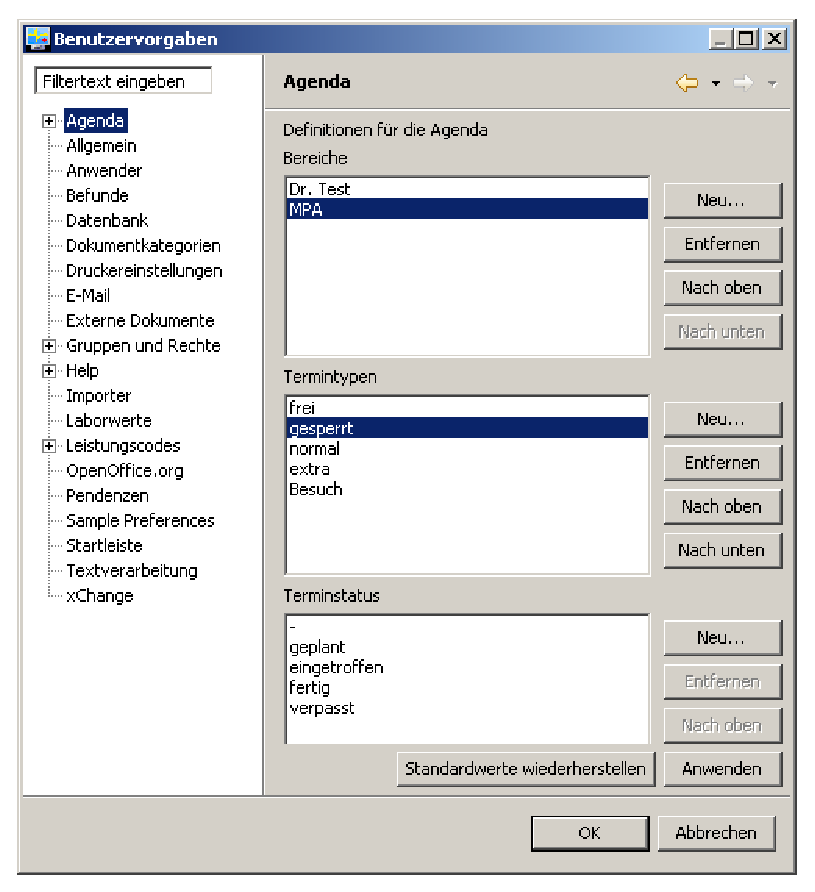
\includegraphics[width=3in,bb=0 0 382 420]{images/settings1}
% settings1.jpg: 499x548 pixel, 94dpi, 13.49x14.81 cm, bb=0 0 382 420

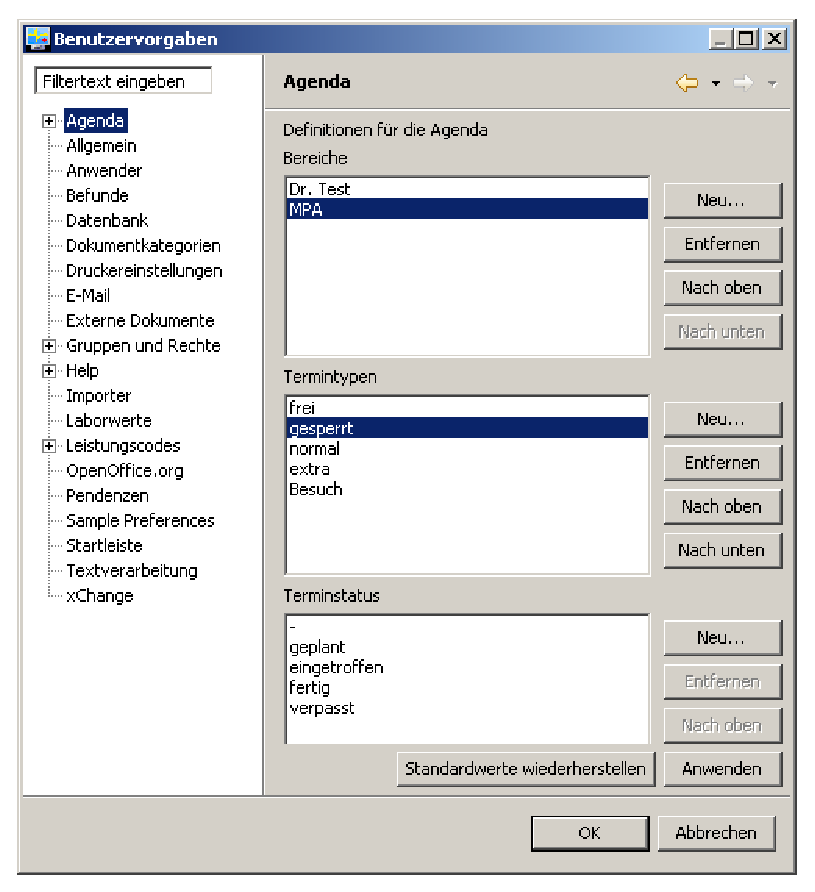
\includegraphics{images/settings1}

Im oberen Abschnitt \textit{Bereiche} \index{Agenda!Bereich} können Sie angeben,
wieviele und welche Agenden parallel geführt werden sollen.
Dies kann beispielsweise eine eigene Agenda für jeden Arzt einer
\index{Gemeinschaftspraxis} Gemeinschaftspraxis, oder auch bestimmte Ressourcen sein (z.B. Arzt, EKG, Labor, Ergometrie etc.).
Menge und Titel der Bereiche sind ganz von den spezifischen Bedürfnissen Ihrer Praxis abhängig.

Darunter,\textit{Termintypen} \index{Agenda!Termintyp} können Sie angeben, welche
verschiedene Arten von Terminen es bei Ihnen geben soll. Ein Termintyp ist alles, was eingetragen werden kann. Also beispielsweise auch  \textit{Teamsitzung},  \textit{Akupunktur},  \textit{Check-Up},  \textit{Fortbildung}  usw. Termintypen werden später unterschiedlich angezeigt und können unterschiedliche Zeitvorgaben haben. Die ersten beiden Einträge, frei und gesperrt, müssen mit dieser Bedeutung in dieser Reihenfolge angegeben sein, dürfen aber anders genannt werden (z.B. \textit{leer}  und  \textit{reserviert}). Die anderen Zeilen können Sie beliebig benennen und es können beliebig viele sein.

Das unterste Feld, \textit{Terminstatus}\index{Agenda!Terminstatus}, ist ebenfalls ganz von den spezifischen
Gegebenheiten Ihrer Praxis abhängig. Auch hier sind die zwei obersten Einträge in ihrer Bedeutung vorgegeben
(können aber anders benannt werden), während die anderen völlig frei sind. Man könnte hier z.B.
auch  \textit{abgesagt}, \textit{wartet auf Labor}, \textit{wartet auf Arzt}  etc. eingeben.

Die nächste Einstellungsseite der Agenda betrifft die Icons\index{Agenda!Icons}, mit denen die verschiedenen Termintypen angezeigt werden sollen.

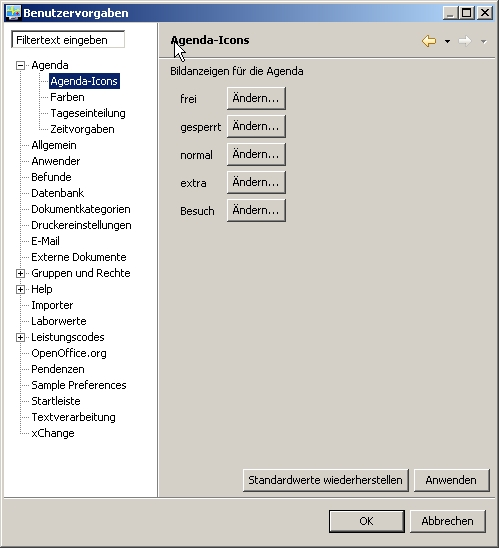
\includegraphics[width=3in]{images/settings2}

(Falls hier noch nicht Ihre gewählten Termintypen auftauchen, müssen Sie Elexis beenden und neu starten, um sie korrekt einzulesen).
Klicken Sie auf  \textit{Ändern} und wählen Sie ein Bild im .*gif, *png oder *.ico Format aus.

Der nächste Abschnitt betrifft die Anzeigefarben für Termintypen und -Status:

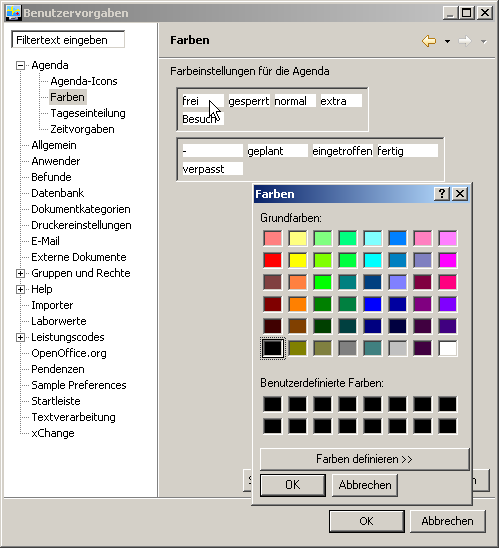
\includegraphics[width=3in]{images/settings3}

Nach Doppelklick auf ein Feld können Sie die Farbe für dieses Feld auswählen.

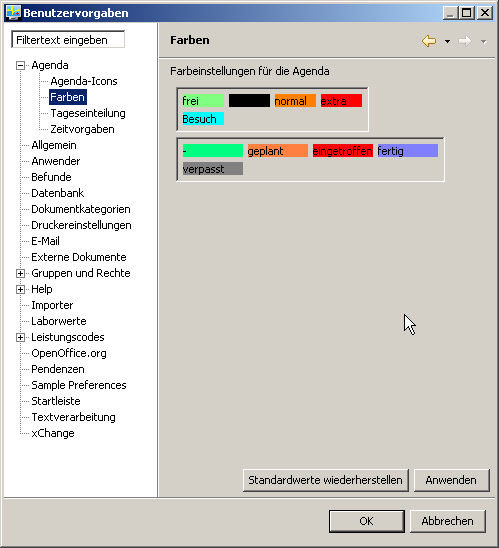
\includegraphics[width=3in]{images/settings4.png}


Die obere Reihe betrifft die Termintypen. Die hier angezeigten Farben werden im Termineingabedialog angezeigt.
Die untere Reihe ist der Terminstatus; diese Farben werden in der normalen Agenda-Anzeige dargestellt

Der nächste Abschnitt der Agenda-Einstellungen betrifft die Tageseinteilung\index{Tageseinteilung}:

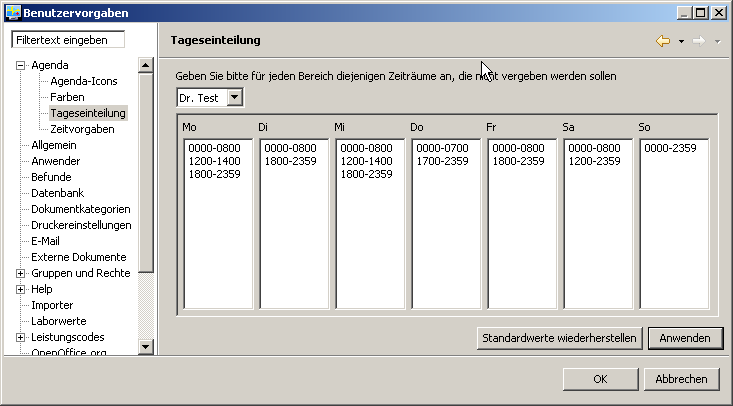
\includegraphics[width=3in]{images/settings5.png}
% settings5.png: 733x406 pixel, 96dpi, 19.39x10.74 cm, bb=0 0 550 304

Hier wird eingestellt, welche Zeiträume für jeden Wochentag standardmässig für jeden Agenda-Bereich planbar sind. Dies kann
nachträglich natürlich für jeden Tag auch separat geändert werden; hier geht es um die Vorgaben.

Wählen Sie oben den gewünschten Bereich, und geben Sie hier jeweils Beginn- und Ende für jeden nicht
planbaren Zeitraum an. Diese Zeiträume werden später mit dem Termintyp \textit{gesperrt} besetzt. Sie können beliebig viele dieser
Zeiträume für jeden Wochentag \index{Wochentag} eingeben.

Der letzte Abschnitt der Agenda-Einstellungen betrifft die Vorgabe-Zeitdauer für jeden Termintyp:

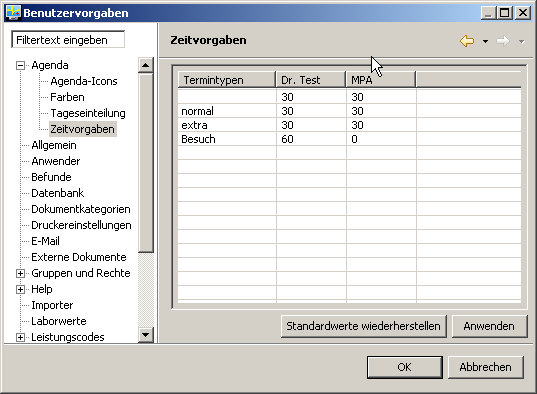
\includegraphics[width=3in]{images/settings6.png}
% settings6.png: 537x394 pixel, 96dpi, 14.21x10.42 cm, bb=0 0 403 295

Hier sehen Sie für jeden Bereich und jeden Termintyp eine Zeitangabe in Minuten.
Sie können jedes Feld durch Anklicken und Überschreiben ändern. Diese Zeit wird die Agenda jeweils standardmässig für die entsprechenden
 Termintypen vorgeben (kann aber jeweils manuell geändert werden). Wenn Sie an einer Stelle 0 eingeben, dann wird dieser Termintyp beim
 entsprechenden Bereich gar nicht angeboten.
Die oberste Zeile ist die Standarddauer, die immer dann angewendet wird, wenn keine spezifische Dauer  gefunden werden kann.

Des weiteren können Sie einige Einstellungen zum Druck von Terminkarten vornehmen.
Diese Einstellungen finden Sie unter \textit{Druck}\index{Agenda!Druck}.

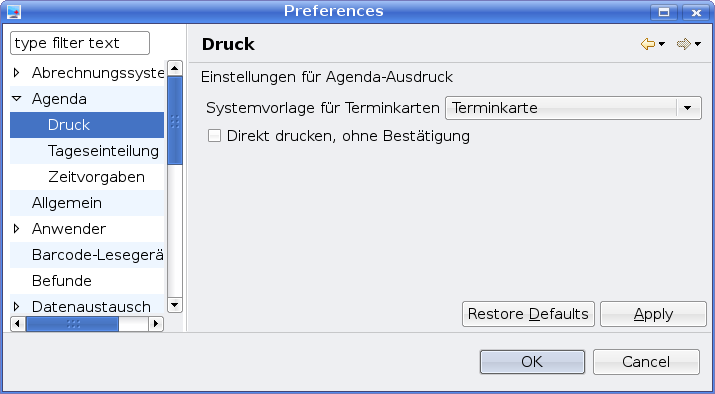
\includegraphics[width=3in]{images/settings-agenda-druck1.png}

Die Standard-Vorlage für den Ausdruck von Terminkarten heisst \textit{Terminkarte}. Sie können
eine beliebige andere Systemvorlage wählen. Die Termine werden beim Platzhalter
\textit{[Termine]} eingesetzt.

Beim Ausdruck einer Terminkarte erscheint ein Fenster mit der vorbereiteten Terminkarte.
Sie können die Terminkarte aus der Textverarbeitung heraus drucken.

Möchten Sie, dass die Terminkarte direkt auf dem Drucker ausgegeben wird, markieren Sie
\textit{Direkt drucken}. Sie können nun den Drucker und optional den gewünschten Schacht
auswählen. Falls Sie keinen Schacht auswählen, wird der in der Vorlage gespeicherte
Schacht oder der Standard-Schacht des ausgewählten Druckers verwendet.

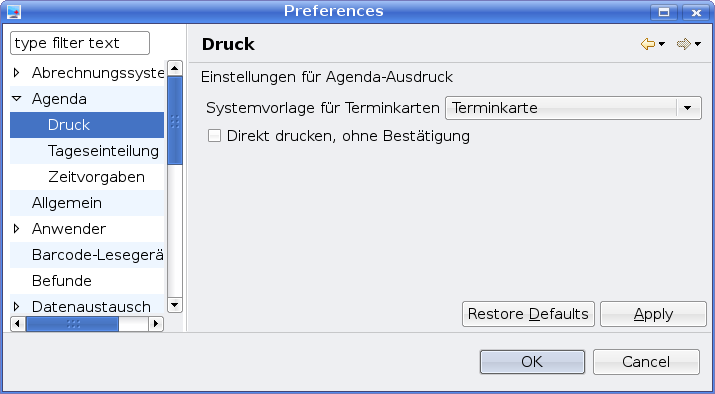
\includegraphics[width=3in]{images/settings-agenda-druck1.png}

Damit sind Sie mit der Konfiguration der Agenda fertig. Drücken Sie auf \textit{OK} und beenden Sie Elexis. Ab dem nächsten Programmstart stehen die neuen Einstellungen zur Verfügung.

Die nächsten Abschnitte befassen sich kurz mit der Bedienung der Agenda.
\subsection{Bedienung der Agenda}

Die Agenda-View (Abb. \ref{fig:agenda1}) wird standardmässig nicht angezeigt. Um sie auf den Bildschirm zu holen, wählen Sie im Menu
 \textbf{Fenster-Ansicht-Andere}, tippen Sie im Filterfeld oben \textit{Agenda}, wählen Sie die Agenda aus und
 klicken Sie \textit{OK}. Ziehen Sie danach das Agenda-Fenster\index{Agenda-Fenster} an die gewünschte Position der Perspektive, wie in \textit{erste Schritte} \ref{tour:customize} auf S. \pageref{tour:customize} beschrieben. 
\begin{wrapfigure}[22]{L}{3in}
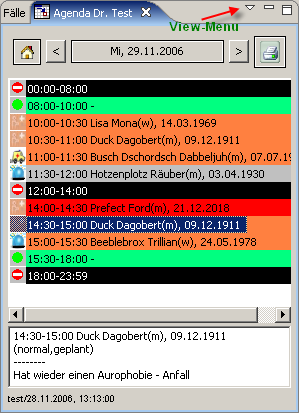
\includegraphics[width=3in]{images/use2.png}
\caption{Agenda-Standardsicht}\label{fig:agenda1}
\end{wrapfigure}
Im Oberen Bereich können Sie das Datum einstellen. Klick auf das Haus führt zum heutigen Tag, Klick auf die Pfeile einen Tag vor oder
zurück, Klick auf den mittleren Bereich zu einem Kalender, auf dem man das Datum auswählen kann.
Klick auf das Dreieck rechts oben öffnet das View-Menu, in dem man den aktuell anzuzeigenden Bereich und die Tagesgrenzen\index{Tagesgrenzen} einstellen kann.

Im Hauptbereich sehen Sie die Agendaeinträge mit den Unter Terminstatus definierten Farben und mit jeweils dem Bild, das für den betreffenden Termintyp definiert wurde. Grün sind die noch freien  Zeiträume. Beachten Sie, dass diese Agenda die Zeiträume nicht proportional zu ihrer Dauer anzeigt. Dies ist zwar am Anfang etwas gewöhnungsbedürftig, aber es hat sich bewährt, da man so auf kleinem Raum den ganzen Tag anzeigen kann

\medskip 

Im untersten Bereich schliesslich sehen Sie weitere Informationen zum aktuell ausgewählten Termin.

\bigskip

Wenn Sie auf einem freien Zeitraum doppelklicken, können Sie einen neuen Termin eingeben, wenn Sie auf einen Termin doppelklicken,
können Sie diesen Termin ändern. In beiden Fällen geht das Dialogfenster Abb. \ref{fig:termineingabe} auf.

\begin{figure}
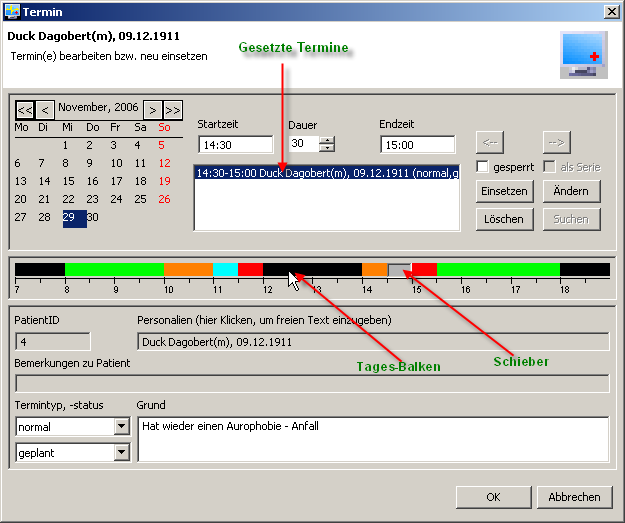
\includegraphics[width=5in]{images/use4.png}
% use4.png: 625x523 pixel, 96dpi, 16.53x13.84 cm, bb=0 0 469 392
\caption{Termineingabe-Dialog}\label{fig:termineingabe}
\end{figure}
Diese recht komplexe Dialogbox ist in mehrere Bereiche unterteilt:

\begin{itemize}
 \item Oben links ein Kalender, in dem sie einen anderen Tag auswählen können
\item Oben in der Mitte Felder für Anfangszeit, Endzeit und Dauer des aktuell ausgewählten Termins,
\item  darunter eine Liste der Termine, die bereits eingesetzt wurden (man kann einen oder mehrere Termine auf einmal einsetzen)
\item Oben rechts eine Checkbox \textit{gesperrt}, diese verhindert spätere Änderungen des Termins,
\item  darunter einen Knopf \textit{einsetzen}, mit der man einen Termin einsetzen kann. Danach kann man einen anderen Tag und/oder andere Zeiten wählen, um einen weiteren Termin in diese Serie einzusetzen. (Wenn man nur einen Termin setzen möchte, kann man stattdessen auch gleich auf OK drücken)
\item Im Mittleren Bereich ist der \textit{Tagesbalken}, welcher die Aufteilung des aktuell ausgewählten Tages anzeigt. Die Farben entsprechen den Termintypen, wie Sie sie in der Konfiguration eingegeben haben. Der graue Schieber symbolisiert den aktuell eingestellten Zeitraum. Sie können den Schieber mit der Maus beliebig hin- und herziehen.
\item Die Uhrzeiten-Anzeige unterhalb des Tagesbalkens gibt das Raster vor, in dem der Schieber verschoben werden kann,. Durch Anklicken dieser Zeile können Sie das Raster verändern.


\item Darunter sind schliesslich die Personalien des ausgewählten Patienten, sowie Typ, Status und Text zum aktuellen Termin.
Wenn Sie nicht einen Patienten, sondern freien Text eingeben wollen, können Sie auf die Zeile \textit{Personalien} klicken und können dann selbst die Angaben verändern.
\end{itemize}

Mit Klick auf OK wird der aktuelle Termin gesetzt und der Dialog wieder geschlossen.


Wenn Sie einen Termin mit der rechten Maustaste anklicken, öffnet sich ein Kontextmenü, in dem Sie verschiedene Details zum Termin ändern können.

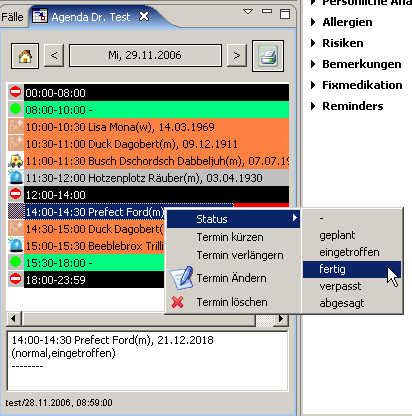
\includegraphics[width=4in]{images/use5.png}
% use5.png: 412x416 pixel, 96dpi, 10.90x11.01 cm, bb=0 0 309 312

Am wichtigsten wohl die Veränderungen des Terminstatus\index{Terminstatus}: Da eine solche Änderung auf alle im Netz angeschlossenen PC's repliziert wird, kann von den anderen Stationen aus festgestellt werden, dass z.B. jemand \textit{eingetroffen} ist.

Wenn Sie für einen einzelnen Tag die reservierten Zeiträume ändern wollen, können Sie im Viewmenü
oben \textit{Tagesgrenzen} auswählen. Es erscheint dann folgender Dialog:

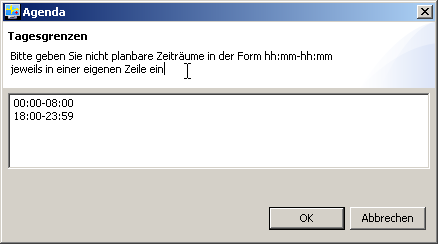
\includegraphics[width=3in]{images/use3.png}
% use3.png: 438x244 pixel, 96dpi, 11.59x6.46 cm, bb=0 0 328 183

Hier können Sie (wie in den Einstellungen beschrieben) für den aktuellen Tag die Sperrzeiten einstellen.

\subsubsection{Mehrere Agendafenster gleichzeitig}
Sie können ohne weiteres auch mehrere Agendafenster gleichzeitig darstellen, um etwa verschiedene Bereiche oder verschiedene Tage anzuzeigen.

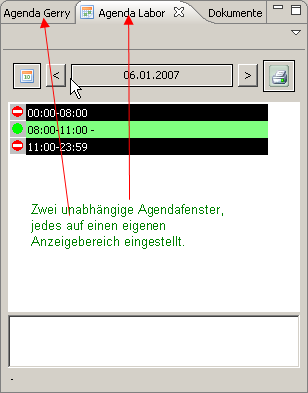
\includegraphics[width=3in]{images/agendamulti.png}
% agendamulti.png: 308x393 pixel, 96dpi, 8.15x10.40 cm, bb=0 0 231 295

\subsubsection{Grösseres Fenster}

Ihre MPA möchte vielleicht auf ihrem Bildschirm eine Agenda, die mehr Informationen auf einen Blick liefert. Hierfür ist die View \textit{Agenda gross} geeignet:

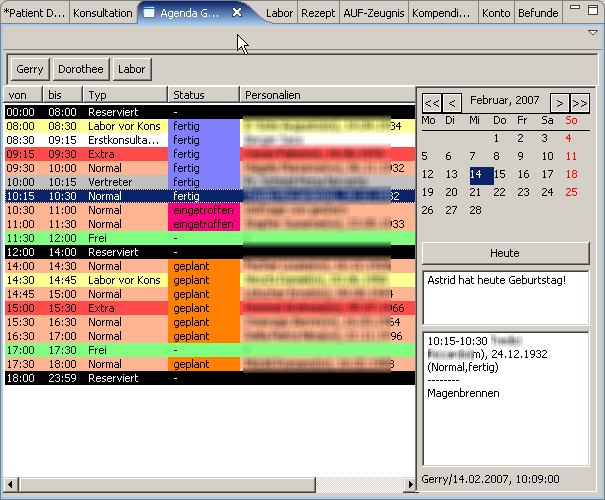
\includegraphics[width=5in]{images/agenda2.png}
% agenda2.png: 605x500 pixel, 96dpi, 16.01x13.23 cm, bb=0 0 454 375

Wie Sie sehen, werden hier alle relevanten Informationen synoptisch dargestellt. Ansonsten ist die Funktion genau identisch;
Sie können ohne weiteres auch beide Agenda-Viewtypen gleichzeitig benutzen

\subsubsection{Terminkarten drucken}

Im View-Menü der Agenda können Sie \textit{Patienten-Termine drucken} wählen, um eine Terminkarte
für den ausgewählten Patienten zu drucken. Die Zugehörige Formatvorlage heisst \textit{Terminkarte}.
Weitere Informationen zur Konfiguration finden Sie weiter oben.

Beim Ausdruck einer Terminkarte erscheint ein Fenster mit der vorbereiteten Terminkarte.
Sie können die Terminkarte aus der Textverarbeitung heraus drucken. Das Fenster können Sie
danach durch Klicken auf \textit{OK} oder \textit{Abbrechen} wieder schliessen.

